\documentclass{beamer}
\usetheme{default}
\usecolortheme{seahorse}
\setbeamertemplate{navigation symbols}{}
\setbeamertemplate{items}[ball]
\setbeamertemplate{footline}[frame number]
\setbeamertemplate{section in toc}[ball]
\setbeamerfont{section in toc}{series=\bfseries}
\renewcommand{\arraystretch}{1.25}

\usepackage[fontset=none]{ctex}
\setCJKsansfont{SimSun}[BoldFont=Noto Sans CJK SC Medium]
\usepackage{amsmath,amssymb,mathrsfs,bm}
\usepackage{tikz}
\usepackage{anyfontsize}
\usepackage{unicode-math}
\unimathsetup{mathrm=sym,bold-style=ISO,sans-style=italic}
\renewcommand{\bm}{\symbf}
\renewcommand{\mathsf}{\symsf}
\setmathfont{Latin Modern Math}
\usepackage{fontspec}
\usefonttheme[onlymath]{serif}
\usepackage{color}
\usepackage{graphicx,caption,subcaption}
\usepackage{hyperref}
\hypersetup{
    colorlinks=true,
    linkcolor=blue,
    filecolor=green,
    urlcolor=cyan,
    citecolor=cyan,
}

\AtBeginDocument{
  \let\uglyepsilon\epsilon
  \renewcommand\epsilon{\varepsilon}
}
\AtBeginDocument{
  \let\uglymathsf\mathsf
  \renewcommand\mathsf{\symsf}
}

\let\sectiononly\section
\renewcommand{\section}[1]{
    \sectiononly{#1}
    \let\sectiontitle\relax
    \newcommand{\sectiontitle}{#1}
}

\newenvironment{slide}{
    \begin{frame}{\bfseries{\sectiontitle}}
}{
    \end{frame}
}

\title{\textbf{简单复习}}\thispagestyle{empty}
\author{江林华}
\date{\today}

\begin{document}

\begin{frame}
    \maketitle
\end{frame}

\begin{frame}{\textbf{目录}}\thispagestyle{empty}
    \tableofcontents
\end{frame}

\section{热动平衡下的统计函数和统计方程}

\begin{slide}
    \addtocounter{framenumber}{-2}
    \begin{itemize}
        \item 热力学系统
        \item Boltzmann分布
        \item Bose-Einstein分布和Fermi-Dirac分布
        \item Boltzmann方程
        \item Maxwell分布
    \end{itemize}
\end{slide}

\begin{slide}
    \begin{itemize}
        \item \textbf{热力学系统}

        全同近独立粒子：$N$、$E$、$V$

        能级：$\epsilon_i$，简并度：$g_i$，各能级的粒子数：$N_i$

        满足条件：$\sum\limits_i N_i=N$，$\sum\limits_i n_i\epsilon_i=E$

        \item \textbf{Boltzmann分布}

        粒子可以分辨，微观状态数：
        \[
            \Omega_{\mathrm{MB}}=\frac{N!}{\prod\limits_i N_i!}\prod_i {g_i}^{N_i}
        \]
        作近似，求偏导，得到\textbf{Boltzmann分布}（最概然分布）：
        \[
            \boxed{
            N_i = \frac{g_i}{\mathrm{e}^{\alpha+\beta\epsilon_i}}\quad
            (\alpha=-\frac{\mu}{kT},\ \beta=\dfrac{1}{kT})
            }
        \]
    \end{itemize}
\end{slide}

\begin{slide}
    \begin{itemize}
        \item \textbf{Bose-Einstein分布}

        粒子不可分辨，一个量子态内可容纳的粒子数不受限制
        \[
            \boxed{
            N_i = \frac{g_i}{\mathrm{e}^{\alpha+\beta\epsilon_i}-1}
            }
        \]
        \item \textbf{Fermi-Dirac分布}

        粒子不可分辨，一个量子态内只能容纳一个粒子
        \[
            \boxed{
            N_i = \frac{g_i}{\mathrm{e}^{\alpha+\beta\epsilon_i}+1}
            }
        \]
        \item \textbf{经典极限}

        如果$\mathrm{e}^{\alpha}\gg1$，或$N_i\ll g_i$，即平均而言每个量子态上的粒子数远小于$1$，则三种分布一样。（一般气体都满足）
    \end{itemize}
\end{slide}

\begin{slide}
    \begin{itemize}
        \item \textbf{Boltzmann方程}

        定义\textbf{配分函数}$Z=\sum\limits_i g_i\mathrm{e}^{-\beta\epsilon_i}$，则由$N_i=g_i\mathrm{e}^{-\alpha-\beta\epsilon_i}$及$N=\sum\limits_i g_i\mathrm{e}^{-\alpha-\beta\epsilon_i}=\mathrm{e}^{-\alpha}Z$，得到\textbf{Boltzmann方程}：
        \[
            \boxed{
            \frac{N_i}{N} = \frac{g_i}{Z}\mathrm{e}^{-\tfrac{\epsilon_i}{kT}}
            }
        \]
        不同能级粒子数比的\textbf{Boltzmann方程}：
        \[
            \boxed{
            \frac{N_i}{N_j} = \frac{g_i}{g_j}\mathrm{e}^{-\tfrac{\epsilon_i-\epsilon_j}{kT}}
            }
        \]
    \end{itemize}
\end{slide}

\begin{slide}
    \begin{itemize}
        \item \textbf{动量矢量的Maxwell分布}

        考虑$N$、$E$、$V$和$n_i=g_i\mathrm{e}^{-\alpha-\beta\epsilon_i}$，相空间单元格大小为$h^3=(\mathrm{d}x\mathrm{d}p_x)(\mathrm{d}y\mathrm{d}p_y)(\mathrm{d}z\mathrm{d}p_z)$

        在$\mathrm{d}p_x\mathrm{d}p_y\mathrm{d}p_z$内的状态数为$g_i=\dfrac{V}{\mathrm{d}x\mathrm{d}y\mathrm{d}z}=\dfrac{V}{h^3}\mathrm{d}p_x\mathrm{d}p_y\mathrm{d}p_z$

        则$\mathrm{d}p_x\mathrm{d}p_y\mathrm{d}p_z$内的粒子数为$f_{\bm{p}}(p_x,p_y,p_z)=\dfrac{V}{h^3}\mathrm{e}^{-\alpha-\beta\epsilon_i}$

        由${\displaystyle\iiint\limits_V f_{\bm{p}}\,\mathrm{d}p_x\mathrm{d}p_y\mathrm{d}p_z}=N$得：$\mathrm{e}^{-\alpha}=\dfrac{N}{V}\left(\dfrac{h^2}{2\pi mkT}\right)^{\tfrac{3}{2}}$

        于是得到\textbf{动量矢量的Maxwell分布}（与$h$无关）：
        \[
            \boxed{
            f_{\bm{p}} = N\left(\dfrac{1}{2\pi mkT}\right)^{\tfrac{3}{2}}\mathrm{e}^{-\tfrac{1}{2mkT}(p_x^2+p_y^2+p_z^2)}
            }
        \]
    \end{itemize}
\end{slide}

\begin{slide}
    \begin{itemize}
        \item \textbf{速度的Maxwell分布}

        由动量矢量的Maxwell分布及$p_x=mv_x$、$p_y=mv_y$、$p_z=mv_z$得\textbf{速度的Maxwell分布}：
        \[
            \boxed{
            f_{\bm{v}} = N\left(\dfrac{m}{2\pi kT}\right)^{\tfrac{3}{2}}\mathrm{e}^{-\tfrac{m}{2kT}(v_x^2+v_y^2+v_z^2)}
            }
        \]
        满足${\displaystyle\iiint\limits_V f_{\bm{v}}\,\mathrm{d}v_x\mathrm{d}v_y\mathrm{d}v_z}=N$
    \end{itemize}
\end{slide}

\begin{slide}
    \begin{itemize}
        \item \textbf{速率的Maxwell分布}

        由速度的Maxwell分布，对方向$(\theta,\varphi)$积分得\textbf{速率的Maxwell分布}：
        \[
            \boxed{
            f_v = 4\pi Nv^2\left(\dfrac{m}{2\pi kT}\right)^{\tfrac{3}{2}}\mathrm{e}^{-\tfrac{m}{2kT}v^2}
            }
        \]
        \item \textbf{某方向速率的Maxwell分布}

        考虑某个方向的速度分量，其大小分布为：
        \[
            f_{v_x} = N\left(\dfrac{m}{2\pi kT}\right)^{\tfrac{1}{2}}\mathrm{e}^{-\tfrac{m}{2kT}v^2}
        \]
    \end{itemize}
\end{slide}

\section{原子电子的能级、跃迁和电离}

\begin{slide}
    \begin{itemize}
        \item 能级
        \item 跃迁和Einstein系数
        \item 电离
        \item 电离原子的Boltzmann方程
        \item Saha方程
    \end{itemize}
\end{slide}

\begin{slide}
    \begin{itemize}
        \item \textbf{能级}

        能级$j$高于能级$i$，能量差为：$\epsilon_{ij}=\epsilon_j-\epsilon_i=h\nu$

        两个能级上粒子数之比为：$\dfrac{N_i}{N_j} = \dfrac{g_i}{g_j}\mathrm{e}^{-\tfrac{h\nu}{kT}}$

        \item \textbf{跃迁和Einstein系数}

        电子会自发从高能级向低能级\textbf{跃迁}：
        \begin{itemize}
            \item 单位时间$\mathrm{d}t$内自发跃迁的电子个数：$A_{ji}N_j\mathrm{d}t$

            \item 外加辐射场$I_\nu$：$B_{ji}N_jI_\nu\mathrm{d}t$

            \item 吸收：$B_{ij}N_iI_\nu\mathrm{d}t$
        \end{itemize}

        比例系数$A_{ji}$、$B_{ji}$、$B_{ij}$被称为\textbf{Einstein系数}，满足如下的热动平衡条件：
        \[
            \boxed{
            N_j(A_{ji}+B_{ji}I_\nu) = N_iB_{ij}I_\nu
            }
        \]
    \end{itemize}
\end{slide}

\begin{slide}
    \begin{itemize}
        \item \textbf{跃迁和Einstein系数}

        由Boltzmann分布得：
        \[
            I_\nu = \frac{g_jA_{ji}}{g_iB_{ij}\mathrm{e}^{\tfrac{h\nu}{kT}}-g_jB_{ji}}
        \]
        因为$T\to\infty$时$I_\nu\to\infty$，所以$\boxed{g_iB_{ij}=g_jB_{ji}}$

        化简得：$I_\nu = \left(\dfrac{A_{ji}}{B_{ji}}\right)\mathrm{e}^{-\tfrac{h\nu}{kT}}$

        热动平衡下，对于黑体有：$I_\nu = B_\nu = \left(\dfrac{2h\nu^3}{c^2}\right)\mathrm{e}^{-\tfrac{h\nu}{kT}}$

        对比可得：$\boxed{\dfrac{A_{ji}}{B_{ji}} = \dfrac{2h\nu^3}{c^2}}$
    \end{itemize}
\end{slide}

\begin{slide}
    \begin{itemize}
        \item \textbf{电离}
        \begin{itemize}
            \item 用$\chi_r$表示$r$次电离的原子再电离一个电子的\textbf{电离电势}

            \item 用$\epsilon_{r,k}$表示$r$次电离原子在$k$能级的\textbf{激发电势}

            \item 把原子从某个激发能级电离所需要的最小能量称为该能级的\textbf{结合能}，用$\chi_{r,k}$表示，它和电离电势$\chi_r$的关系是：
            \[
                \chi_r = \chi_{r,k} + \epsilon_{r,k}
            \]
            $\chi_{0,1}$表示中性（电离度$r=0$）基态（能级$k=0$）的原子
        \end{itemize}

        原子从能级$\chi_{r,k}$出发，吸收了能量$h\nu\geqslant\chi_{r,k}$的光子，则会发生\textbf{光致电离}，这时电子获得剩余动能$E_k$，满足\textbf{Einstein光电效应方程}：（$m_e$为电子质量）
        \[
            \boxed{
            h\nu = \chi_{r,k} + E_k = \chi_{r,k} + \frac{1}{2}m_ev^2
            }
        \]
    \end{itemize}
\end{slide}

\begin{slide}
    \begin{itemize}
        \item \textbf{电离原子的Boltzmann方程}

        设$r$次电离的原子总数为$N_r=\sum\limits_i N_{r,i}$

        相应的配分函数为$Z_r=\sum\limits_i N_{r,i}\mathrm{e}^{-\tfrac{\epsilon_{r,i}}{kT}}$

        则有\textbf{电离原子的Boltzmann方程}：
        \[
            \boxed{
            \frac{N_{r,i}}{N_r} = \frac{g_{r,i}}{Z_r}\mathrm{e}^{-\tfrac{\epsilon_{r,i}}{kT}},\quad
            \frac{N_{r,j}}{N_{r,i}} = \frac{g_{r,j}}{g_{r,i}}\mathrm{e}^{-\tfrac{\epsilon_{r,i}-\epsilon_{r,j}}{kT}}
            }
        \]
        后者写成常用对数形式得：
        \[
            \lg\frac{N_{r,j}}{N_{r,i}} = \lg\frac{g_{r,j}}{g_{r,i}} - (\epsilon_{r,i}-\epsilon_{r,j})\frac{5040}{T}
        \]
        这里的$\epsilon_{r,i}$和$\epsilon_{r,j}$单位为$\mathrm{eV}$，$5040$为$\dfrac{e}{k\ln10}$的近似值
    \end{itemize}
\end{slide}

\begin{slide}
    \begin{itemize}
        \item \textbf{电离原子的Boltzmann方程}

        例如，对于中性氢原子，$r=0$，$i=1$，$j=2$：
        \begin{center}
            \begin{tabular}{|c|c|c|c|}
                \hline
                $T/\mathrm{K}$ & $6\times10^{3}$ & $1.0\times10^{4}$ & $1.5\times10^{4}$ \\
                \hline
                $N_{r,2}/N_{r,1}$ & $1.0\times10^{-8}$ & $3.1\times10^{-5}$ & $1.55\times10^{-3}$ \\
                \hline
            \end{tabular}
        \end{center}
        可见在恒星表面依然以氢的基态为主，且随表面温度的降低，激发态氢的比例迅速减小
    \end{itemize}
\end{slide}

\begin{slide}
    \begin{itemize}
        \item \textbf{Saha方程}

        从Boltzmann方程推导Saha方程如下（这里用分子数密度$n$代替分子数$N$）：
        \[
            \frac{n_i}{n_j} = \frac{g_i}{g_j}\mathrm{e}^{-\tfrac{\Delta E}{kT}}
        \]

        考虑一个$r$级电离原子再电离一个电子变为$r+1$级电离原子的过程：
        \begin{itemize}
            \item $g_i$分为两部分：$r+1$级电离原子的统计权$g_{r+1}$和自由电子的统计权$g_e$，且$g_i=g_{r+1}g_e$

            \item $g_j$即为$r$级电离原子的统计权$g_{r}$

            \item 能量差$\Delta E$为电子相对于$r$级电离原子的能量
        \end{itemize}

    \end{itemize}
\end{slide}

\begin{slide}
    \begin{itemize}
        \item \textbf{Saha方程}

        自由电子的微观状态数，即电子的统计权重$g_e$为：（因子$2$是由于每个相格中可容纳自旋方向相反的两个电子）
        \[
            g_e = \frac{2\mathrm{d}^3q\mathrm{d}^3p}{h^3}
        \]
        将动量对方向积分：$\mathrm{d}^3p=4\pi p^2\mathrm{d}p$，并代入一个电子所占体积$\mathrm{d}^3q=V_e=n_e^{-1}$（$n_e$为电子的数密度），得到动量大小在$p\sim p+\mathrm{d}p$内，电子的微观状态数为：
        \[
            g_e = \frac{V_e4\pi p^2\mathrm{d}p}{h^3} = \frac{4\pi p^2\mathrm{d}p}{n_eh^3}
        \]
        电子相对于$r$级电离原子的能量$\Delta E=\chi_{r}+\dfrac{p^2}{2m_e}$
    \end{itemize}
\end{slide}

\begin{slide}
    \begin{itemize}
        \item \textbf{Saha方程}

        代入Boltzmann方程得：
        \[
            \frac{n_{r+1}}{n_r} = \frac{g_{r+1}}{g_r}\cdot\frac{2}{n_eh^3}\int_0^{\infty}\mathrm{e}^{-\tfrac{1}{kT}\left(\chi_r-\tfrac{p^2}{2m_e}\right)}4\pi p^2\,\mathrm{d}p
        \]
        积分即得\textbf{Saha方程}：
        \[
            \boxed{
            \frac{n_{r+1}n_e}{n_r} = \frac{2g_{r+1}}{g_r}\left(\frac{2\pi m_ekT}{h^2}\right)^{\tfrac{3}{2}}\mathrm{e}^{-\tfrac{\chi_r}{kT}}
            }
        \]
        Saha方程描述的是\textbf{不同电离态下的分布}，而Boltzmann方程描述的是同一电离态下不同能级的分布
    \end{itemize}
\end{slide}

\begin{slide}
    \begin{itemize}
        \item \textbf{Saha方程}

        其中：
        \[
            \boxed{
            Z_e = 2\left(\frac{2\pi m_ekT}{h^2}\right)^{\tfrac{3}{2}}
            }
        \]
        被称为\textbf{电子配分函数}

        在SI单位制下：$Z_e\approx4.8294\times10^{21}T^{\tfrac{3}{2}}$

        在CGS单位制下$Z_e\approx4.8294\times10^{15}T^{\tfrac{3}{2}}$
    \end{itemize}
\end{slide}

\section{辐射场的宏观描述和辐射转移}

\begin{slide}
    \begin{itemize}
        \item 辐射场
        \item 吸收与光学厚度
        \item 辐射转移方程
        \item 源函数
        \item 亮温度与激发温度
    \end{itemize}
\end{slide}

\begin{slide}
    \begin{itemize}
        \item \textbf{辐射场}

        辐射强度$I_\nu(\bm{r},\bm{k},t)$，注意$I_\nu\mathrm{d}\nu=-I_\lambda\mathrm{d}\lambda$
        \begin{center}
            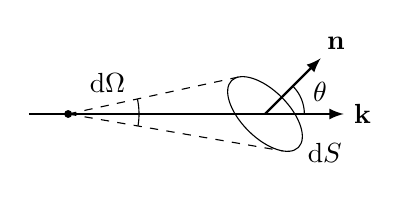
\begin{tikzpicture}
                \fill (-1.5,0) circle [radius=0.05cm];
                \draw (1,0) ellipse [x radius=0.6cm, y radius=0.3cm, rotate=135];
                \draw (1.75,-0.5) node {$\mathrm{d}S$};
                \draw (1,0)--(1.7071068,0.7071068) [thick,->,>=latex];
                \draw (1.5,0) arc [start angle=0,end angle=45,radius=0.5];
                \draw (1.7,0.275) node {$\theta$};
                \draw (1.9,0.9) node {$\bm{n}$};
                \draw (-2,0)--(2,0) [thick,->,>=latex] node[right] {$\bm{k}$};
                \draw (-1.5,0)--(0.66109277,0.46884539) [dashed];
                \draw (-1.5,0)--(1.22370723,-0.46884539) [dashed];
                \draw (-0.6130445,-0.1526761) arc [start angle=-9.76689471,end angle=12.24053431,radius=0.9];
                \draw (-1,0.4) node {$\mathrm{d}\Omega$};
            \end{tikzpicture}
        \end{center}
        单位辐射能量：$\mathrm{d}E_\nu=I_\nu\cos\theta\,\mathrm{d}S\,\mathrm{d}t\,\mathrm{d}\nu\,\mathrm{d}\Omega$

        平均辐射：（对立体角做平均）
        \[
            J_\nu = \frac{1}{4\pi}\int I_\nu\,\mathrm{d}\Omega
        \]
    \end{itemize}
\end{slide}

\begin{slide}
    \begin{itemize}
        \item \textbf{辐射场}

        辐射流量：
        \[
            F_\nu = \int \frac{\mathrm{d}E_\nu}{\mathrm{d}S\mathrm{d}t\mathrm{d}\nu} = \int I_\nu\cos\theta\,\mathrm{d}\Omega
        \]
        辐射流量密度：
        \[
            u_\nu = \frac{1}{c}\int I_\nu\,\mathrm{d}\Omega = \frac{4\pi}{c}J_\nu
        \]
    \end{itemize}
\end{slide}

\begin{slide}
    \begin{itemize}
        \item \textbf{辐射场}

        辐射压$p_\nu$推导如下：

        考虑在时间$(t,\ t+\mathrm{d}t)$、立体角$\mathrm{d}\Omega$内，以与法线方向成$\theta$角射入某一面元$\mathrm{d}S$的频率为$(\nu,\ \nu+\mathrm{d}\nu)$的光，沿面元法向的能量传递为：
        \[
            \mathrm{d}E_{\bm{n}} = \mathrm{d}E\cos\theta = I(\nu)\cos^2\theta\,\mathrm{d}\Omega\,\mathrm{d}t\,\mathrm{d}S\,\mathrm{d}\nu
        \]
        这里的$\cos^2\theta$中，一个$\cos\theta$来源于辐射只有$\cos\theta$的比例投影到表面，另一个$\cos\theta$则是因为辐射压力垂直于表面的分量是$\cos\theta$

        对所有方向$\mathrm{d}\Omega$积分得到（单位频率的）辐射压为：
        \[
            p_\nu = \int \left(\frac{\mathrm{d}E}{c\mathrm{d}t\,\mathrm{d}S\,\mathrm{d}\nu}\right)\mathrm{d}\Omega = \frac{1}{c}\int I_\nu\cos^2\theta\,\mathrm{d}\Omega
        \]
    \end{itemize}
\end{slide}

\begin{slide}
    \begin{itemize}
        \item \textbf{辐射场}

        $\cos\theta$在很多地方都出现，定义$\mu=\cos\theta$

        则单位立体角（假设$\phi$方向对称）$\mathrm{d}\Omega=2\pi\sin\theta\,\mathrm{d}\theta=2\pi\,\mathrm{d}\mu$

        Eddington引入$J$、$H$、$K$三个量描述辐射场，其中：
        \[
            J=\int_{-1}^1 I(\mu)\,\mathrm{d}\mu
        \]
        即为平均辐射，而：
        \[
            H = \frac{1}{2}\int_{-1}^{1} I(\mu)\mu\,\mathrm{d}\mu,\quad
            K = \frac{1}{2}\int_{-1}^{1} I(\mu)\mu^2\,\mathrm{d}\mu
        \]
        则辐射流量$F=4\pi H$，辐射压$p=\dfrac{4\pi}{c}K$
    \end{itemize}
\end{slide}

\begin{slide}
    \begin{itemize}
        \item \textbf{辐射强度与辐射源的距离无关}

        辐射在真空中传播，即反射和吸收均为零时，辐射强度是一个恒量，与辐射源的距离无关，推导如下：
        \begin{center}
            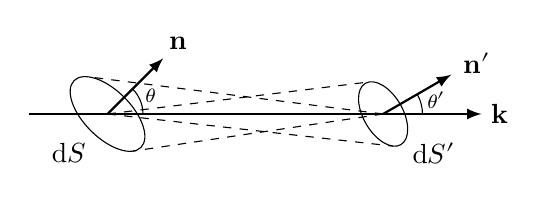
\begin{tikzpicture}
                \draw (-3,0)--(2.75,0) [thick,->,>=latex] node[right] {$\bm{k}$};
                \draw (-2,0) ellipse [x radius=0.6cm, y radius=0.3cm, rotate=135];
                \draw (-2.5,-0.5) node {$\mathrm{d}S$};
                \draw (-2,0)--(-1.2928932,0.7071068) [thick,->,>=latex];
                \draw (-1.55,0) arc [start angle=0,end angle=45,radius=0.45];
                \draw (-1.45,0.225) node {$\scriptstyle\theta$};
                \draw (-1.1,0.9) node {$\bm{n}$};
                \draw (-2,0)--(1.33074646,0.40800348) [dashed];
                \draw (-2,0)--(1.62607657,-0.40800348) [dashed];
                \draw (1.5,0) ellipse [x radius=0.45cm, y radius=0.25cm, rotate=120];
                \draw (2.15,-0.5) node {$\mathrm{d}S'$};
                \draw (1.5,0)--(2.3660254,0.5) [thick,->,>=latex];
                \draw (2,0) arc [start angle=0,end angle=30,radius=0.5];
                \draw (2.175,0.175) node {$\scriptstyle\theta'$};
                \draw (2.7,0.65) node {$\bm{n}'$};
                \draw (1.5,0)--(-2.24178441,0.47154544) [dashed];
                \draw (1.5,0)--(-1.67592988,-0.47154544) [dashed];
            \end{tikzpicture}
        \end{center}
        考虑真空中穿过相距为$d$的两个面元$\mathrm{d}S$和$\mathrm{d}S'$，沿方向$\bm{k}$传播的辐射：
        \[
            \mathrm{d}E_\nu = I_\nu(\bm{r},t,\bm{k})\cos\theta\,\mathrm{d}S\,\mathrm{d}t\,\mathrm{d}\nu\,\mathrm{d}\Omega'
        \]
        \[
            \mathrm{d}E'_\nu = I'_\nu(\bm{r}',t',\bm{k})\cos\theta'\,\mathrm{d}S'\,\mathrm{d}t\,\mathrm{d}\nu\,\mathrm{d}\Omega
        \]
    \end{itemize}
\end{slide}

\begin{slide}
    \begin{itemize}
        \item \textbf{辐射强度与辐射源的距离无关}

        \begin{center}
            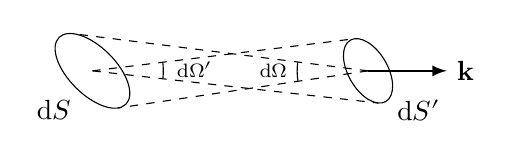
\begin{tikzpicture}
                \draw (1.5,0)--(2.5,0) [thick,->,>=latex] node[right] {$\bm{k}$};
                \draw (-2,0) ellipse [x radius=0.6cm, y radius=0.3cm, rotate=135];
                \draw (-2.5,-0.5) node {$\mathrm{d}S$};
                \draw (-2,0)--(1.33074646,0.40800348) [dashed];
                \draw (-2,0)--(1.62607657,-0.40800348) [dashed];
                \draw (-1.10564375,-0.10063248) arc [start angle=-6.41988742,end angle=6.98371779,radius=0.9];
                \draw (-0.7,0.02) node {$\scriptstyle\mathrm{d}\Omega'$};
                \draw (1.5,0) ellipse [x radius=0.45cm, y radius=0.25cm, rotate=120];
                \draw (2.15,-0.5) node {$\mathrm{d}S'$};
                \draw (1.5,0)--(-2.24178441,0.47154544) [dashed];
                \draw (1.5,0)--(-1.67592988,-0.47154544) [dashed];
                \draw (0.60706263,0.11252934) arc [start angle=172.81736135,end angle=188.44527997,radius=0.9];
                \draw (0.3,0) node {$\scriptstyle\mathrm{d}\Omega$};
            \end{tikzpicture}
        \end{center}
        如图，相对于光传播的方向$\bm{k}$有：
        \[
            \mathrm{d}\Omega' = \frac{\mathrm{d}S'\cos\theta'}{d^2},\quad \mathrm{d}\Omega = \frac{\mathrm{d}S\cos\theta}{d^2}
        \]
        则$\mathrm{d}E_\nu = \mathrm{d}E'_\nu$，即通过两个面元的辐射强度相等：
        \[
            I_\nu(\bm{r},t,\bm{k}) = I'_\nu(\bm{r}',t',\bm{k})
        \]
    \end{itemize}
\end{slide}

\begin{slide}
    \begin{itemize}
        \item \textbf{吸收与光学厚度}

        若只考虑吸收，则满足如下方程：
        \[
            \boxed{
            \mathrm{d}I = -\kappa\rho I\,\mathrm{d}z = -n\sigma I\,\mathrm{d}z
            }
        \]
        其中$\kappa=\kappa(\nu)$为质量吸收系数，它与单个粒子的吸收截面$\sigma$的关系为$\kappa\rho=n\sigma$，其中$\rho$为质量密度，$n$为数密度

        定义\textbf{光学厚度}（\textbf{光深}）：
        \[
            \boxed{
            \tau=\int n\sigma\,\mathrm{d}z
            }
        \]
        即$\mathrm{d}\tau=n\sigma\,\mathrm{d}z$，于是有$\dfrac{\mathrm{d}I}{I}=-\mathrm{d}\tau$，则$I=I_0\mathrm{e}^{-\tau}$
    \end{itemize}
\end{slide}

\begin{slide}
    \begin{itemize}
        \item \textbf{辐射转移方程}

        考虑吸收和发射，则满足如下方程：
        \[
            \mathrm{d}I = -\kappa\rho I\,\mathrm{d}z + j\rho\,\mathrm{d}z
        \]
        其中$j=j(\nu)$为\textbf{发射系数}。

        又因为$\mathrm{d}\tau=-\kappa\rho\,\mathrm{d}z$（负号表示$\tau$的增长方向与$z$相反），两式相除得\textbf{辐射转移方程}：
        \[
            \boxed{
            \frac{\mathrm{d}I}{\mathrm{d}\tau} = I - \frac{j}{\kappa} = I - S
            }
        \]
        其中$\boxed{S=S(\nu)=\dfrac{j(\nu)}{\kappa(\nu)}}$称为\textbf{源函数}
    \end{itemize}
\end{slide}

\begin{slide}
    \begin{itemize}
        \item \textbf{辐射转移方程}

        求解辐射转移方程如下：
        \[
            \frac{\mathrm{d}I}{\mathrm{d}\tau}\mathrm{e}^{-\tau} - I\mathrm{e}^{-\tau} = \frac{\mathrm{d}}{\mathrm{d}\tau}(I\mathrm{e}^{-\tau}) = -S\mathrm{e}^{-\tau}
        \]
        积分得：
        \[
            I(\tau_2) = I(\tau_1)\mathrm{e}^{-(\tau_1-\tau_2)} - \mathrm{e}^{\tau_2}\int_{\tau_1}^{\tau_2}S(\tau)\mathrm{e}^{-\tau}\,\mathrm{d}\tau
        \]
        考虑$\tau_2=0$（天体表面），$\tau_1=\tau_{\mathrm{max}}$，则：
        \[
            I(\tau=0) = I(\tau_{\mathrm{max}})\mathrm{e}^{-\tau_{\mathrm{max}}} + \int_{0}^{\tau_{\mathrm{max}}}S(\tau)\mathrm{e}^{-\tau}\,\mathrm{d}\tau
        \]
    \end{itemize}
\end{slide}

\begin{slide}
    \begin{itemize}
        \item \textbf{辐射转移方程}

        平面平行层大气中，设光线与大气层法线方向的夹角为$\theta$，辐射转移方程变为：
        \[
            \cos\theta\frac{\mathrm{d}I}{\mathrm{d}\tau} = I - S
        \]
        这里的$\mathrm{d}\tau$沿大气层法线方向（即恒星半径方向）

        球坐标中，辐射转移方程变为：
        \[
            \cos\theta\frac{\partial I}{\partial r} - \frac{\sin\theta}{r}\frac{\partial I}{\partial\theta} = -I\kappa\rho + j\rho
        \]
        代入$\mu=\cos\theta$和$\mathrm{d}\tau=-\kappa\rho\mathrm{d}r$得：
        \[
            \mu\frac{\partial I}{\partial\tau} - \frac{(1-\mu^2)}{\tau}\frac{\partial I}{\partial\mu} = I - S
        \]
    \end{itemize}
\end{slide}

\begin{slide}
    \begin{itemize}
        \item \textbf{源函数}

        首先对于恒星大气可以采用\textbf{热动平衡}或\textbf{局部热动平衡}假设：
        \begin{itemize}
            \item 场内各点温度$T$相同，而且是不变的

            \item 热辐射的强度是均匀、各向同性的，其数值由\textbf{Planck辐射定律}决定：
            \[
                \boxed{
                I_\nu(T) = B_\nu(T) = \frac{2h\nu^3}{c^2}\cdot\frac{1}{\mathrm{e}^{\tfrac{h\nu}{kT}}-1}
                }
            \]

            \item 热发射系数和热吸收系数之间的关系满足\textbf{Kirchhoff定律}：
            \[
                \boxed{
                j(\nu) = \kappa(\nu)B_\nu(T)
                }
            \]

            \item 电子的分布、原子的激发和电离可以分别用Boltzmann方程（Maxwell分布）和Saha方程描述
        \end{itemize}
    \end{itemize}
\end{slide}

\begin{slide}
    \begin{itemize}
        \item \textbf{源函数}

        在局部热动平衡假设下：
        \[
            S(\nu) = \frac{j(\nu)}{\kappa(\nu)} = B_\nu(T)
        \]
        如果假设$T$不变（一般不可以），则根据辐射转移方程有：
        \[
            I_\nu(\tau=0) = I_\nu(\tau_{\mathrm{max}})\mathrm{e}^{-\tau_{\mathrm{max}}} + B_\nu(T)(1-\mathrm{e}^{-\tau_{\mathrm{max}}})
        \]
        再假设$\tau_{\mathrm{max}}$很大，则$I_\nu(\tau=0)=B_\nu(T)$，即\textbf{恒星表面可以近似为黑体}

        如果初始没有发射，即$I(\tau_{\mathrm{max}})=0$，则有：
        \[
            I(\tau=0) = B_\nu(1-\mathrm{e}^{-\tau})
        \]
    \end{itemize}
\end{slide}

\begin{slide}
    \begin{itemize}
        \item \textbf{亮温度与激发温度}

        观测到的辐射$I_{\mathrm{obs}}(\nu)$对应的黑体温度为\textbf{亮温度}，在Rayleigh-Jeans近似下为：
        \[
            T_b = \frac{c^2I_{\mathrm{obs}}(\nu)}{2k\nu^2},\quad \frac{h\nu}{kT} \ll 1
        \]
        源函数$S(\nu)$对应的黑体温度为\textbf{激发温度}，在Rayleigh-Jeans近似下为：
        \[
            T_{\mathrm{ex}} = \frac{c^2S(\nu)}{2k\nu^2},\quad \frac{h\nu}{kT} \ll 1
        \]
        对于一个均匀无发射的（光深较大的）云，有：
        \[
            T_b = T_{\mathrm{ex}}(1-\mathrm{e}^{-\tau})
        \]
    \end{itemize}
\end{slide}

\section{氢原子的量子力学描述}

\begin{slide}
    \begin{itemize}
        \item 波函数
        \item Schrödinger方程
        \item 氢原子
        \item 电子分布概率
        \item 能量与角动量
        \item 量子数
        \item 类氢原子
    \end{itemize}
\end{slide}

\begin{slide}
    \begin{itemize}
        \item \textbf{波函数}
        
        考虑平面单色波：
        \[
            \Psi(\bm{r},t) = \Psi_0\mathrm{e}^{i(\bm{k}\cdot\bm{r}-\omega t)}
        \]
        由$p=\hbar k$及$E=\hbar\omega$得：
        \[
            \Psi(\bm{r},t) = \Psi_0\mathrm{e}^{\tfrac{i}{\hbar}(\bm{p}\cdot\bm{r}-Et)}
        \]
        自由粒子的波函数：连续、单值、有限

        \textbf{概率波}：波函数的模方$|\Psi|^2=\Psi\Psi^*$表示在体积$\mathrm{d}V$内发现粒子的几率为$|\Psi|^2\,\mathrm{d}V$，在全空间积分为$1$（\textbf{归一化}）：
        \[
            \iiint |\Psi|^2\,\mathrm{d}V = 1
        \]
    \end{itemize}
\end{slide}

\begin{slide}
    \begin{itemize}
        \item \textbf{Schrödinger方程}
        
        对波函数作用空间Laplace算符得：$\nabla^2\Psi = -\dfrac{p^2}{\hbar}\Psi$

        将波函数对时间$t$求偏导得：$\dfrac{\partial\Psi}{\partial t} = -\dfrac{i}{\hbar}E\Psi$

        又因为对势场$V$中的非相对论粒子有：$E = \dfrac{p^2}{2m} + V$

        联立即得一般的\textbf{Schrödinger方程}：
        \[
            \boxed{
            \left(-\frac{\hbar}{2m}\nabla^2 + V\right)\Psi = i\hbar\frac{\partial\Psi}{\partial t}
            }
        \]
        自由粒子（$V=0$）方程则为：$\boxed{-\dfrac{\hbar}{2m}\nabla^2\Psi = i\hbar\dfrac{\partial\Psi}{\partial t}}$
    \end{itemize}
\end{slide}

\begin{slide}
    \begin{itemize}
        \item \textbf{Schrödinger方程}
        
        考虑势场与时间无关（定态）的情况：
        \[
            \left(-\frac{\hbar}{2m}\nabla^2 + V(\bm{r})\right)\Psi(\bm{r},t) = i\hbar\frac{\partial\Psi(\bm{r},t)}{\partial t}
        \]
        使用分离变量法，令$\Psi(\bm{r},t)=\psi(\bm{r})\varphi(t)$，方程变为：
        \[
            -\frac{\hbar^2}{2m\psi}\nabla^2\psi + V = i\hbar\frac{\mathrm{d}\varphi}{\varphi\,\mathrm{d}t} = E
        \]
        解得$\varphi(t)=\mathrm{e}^{-\tfrac{i}{\hbar}Et}$，则$\psi(\bm{r})$满足\textbf{定态Schrödinger方程}：
        \[
            \boxed{
            \left(-\frac{\hbar}{2m}\nabla^2 + V\right)\psi = E\psi,\quad \Psi = \psi\,\mathrm{e}^{-\tfrac{i}{\hbar}Et}
            }
        \]
    \end{itemize}
\end{slide}

\begin{slide}
    \begin{itemize}
        \item \textbf{Schrödinger方程}
        
        定义表示粒子的总能量的\textbf{Hamilton算符}：
        \[
            \boxed{
            \hat{\mathsf{H}} = -\frac{\hbar}{2m}\nabla^2 + V
            }
        \]
        则一般的Schrödinger方程可以写为：
        \[
            \boxed{
            \hat{\mathsf{H}}\Psi = i\hbar\frac{\partial\Psi}{\partial t}
            }
        \]
        定态Schrödinger方程可以写为：
        \[
            \boxed{
            \hat{\mathsf{H}}\psi = E\psi,\quad \Psi = \psi\,\mathrm{e}^{-\tfrac{i}{\hbar}Et}
            }
        \]
    \end{itemize}
\end{slide}

\begin{slide}
    \begin{itemize}
        \item \textbf{氢原子}
        
        质心系下，$V=-\dfrac{e^2}{4\pi\epsilon_0r}$，得定态Schrödinger方程：
        \[
            \left(-\frac{\hbar}{2\mu}\nabla^2-\frac{e^2}{4\pi\epsilon_0r}\right)\psi(\bm{r}) = E\psi(\bm{r}),\quad \mu = \frac{Mm_e}{M+m_e}
        \]
        分离变量$\psi(r,\theta,\phi)=R(r)Y_{lm}(\theta,\phi)=R(r)\Theta(\theta)\Phi(\phi)$，得到径向和角向方程：
        \[
            \left[-\frac{\hbar^2}{2\mu r^2} \cdot \frac{\mathrm{d}}{\mathrm{d}r}\left(r^2\frac{\mathrm{d}}{\mathrm{d}r}\right) + \frac{\hbar^2l(l+1)}{2\mu r^2} + V(r)\right]R = ER
        \]
        \[
            -\frac{1}{\sin^2\theta}\left[\sin\theta\frac{\partial}{\partial\theta}\left(\sin\theta\frac{\partial}{\partial\theta}\right) + \frac{\partial^2}{\partial\phi^2}\right]Y = l(l+1)Y
        \]
    \end{itemize}
\end{slide}

\begin{slide}
    \begin{itemize}
        \item \textbf{氢原子}
        
        分别求解得：
        \begin{itemize}
            \item $R(r)=R_{nl}(r)$为连带Laguerre函数，其阶数满足：
            \begin{align*}
                n &= 1,\ 2,\ 3,\ \cdots \\
                l &= 0,\ 1,\ \cdots,\ n-1
            \end{align*}
            \item $\Theta(\theta)=\Theta_{ml}(\theta)$为连带Legendre函数，其阶数满足：
            \begin{align*}
                l &= 0,\ 1,\ \cdots,\ n-1 \\
                m &= -l,\ -l+1,\ \cdots,\ l
            \end{align*}
            \item $\Phi(\phi)=\Phi_m(\phi)$为幂函数：$\Phi_m(\phi)=\dfrac{1}{\sqrt{2\pi}}\mathrm{e}^{im\phi}$
        \end{itemize}
    \end{itemize}
\end{slide}

\begin{slide}
    \begin{itemize}
        \item \textbf{电子分布概率}
        
        电子在单位体积$\mathrm{d}V$内分布的概率为：
        \[
            |\psi|^2\,\mathrm{d}V = \left(R^2\Theta^2\Phi\Phi^*\right)r^2\sin\theta\,\mathrm{d}r\mathrm{d}\theta\mathrm{d}\phi
        \]
        其中$R^2r^2\,\mathrm{d}r$、$\Theta^2\sin\theta\,\mathrm{d}\theta$、$\Phi\Phi^*\mathrm{d}\phi$分别表示$r\sim r+\mathrm{d}r$、$\theta\sim\theta+\mathrm{d}\theta$、$\phi\sim\phi+\mathrm{d}\phi$内电子分布的概率

        此处$\Phi\Phi^*=\dfrac{1}{2\pi}$与$\phi$无关，即电子分布关于$\phi$对称
    \end{itemize}
\end{slide}

\begin{slide}
    \begin{itemize}
        \item \textbf{能量与角动量}
        
        \begin{itemize}
            \item \textbf{能量}：由径向方程得能量本征值：
            \[
                E_n = -\left[\frac{\mu}{2\hbar^2}\left(\frac{e^2}{4\pi\epsilon_0}\right)^{\!2}\right]\frac{1}{n^2} = \frac{E_1}{n^2},\quad n = 1,\ 2,\ 3,\ \cdots
            \]
            $E_1$称为基态能量，对于氢原子，$E_1\approx-13.6\,\mathrm{eV}$

            由$E=h\nu$得Rydberg公式：
            \[
                \frac{1}{\lambda} = R\left(\frac{1}{n_f^2}-\frac{1}{n_i^2}\right),\quad R = \frac{\mu}{4\pi c\hbar^3}\left(\frac{e^2}{4\pi\epsilon_0}\right)^{\!2} = \frac{E_1}{hc}
            \]
            $R$称为Rydberg常数，对于氢原子，$R_{\mathrm{H}}\approx1.097\times10^{7}\,\mathrm{m}^{-1}$

            还可以解出Bohr半径$a = \dfrac{4\pi\epsilon_0\hbar^2}{\mu e^2} \approx 0.529\,\symbol{"212B}$
        \end{itemize}
    \end{itemize}
\end{slide}

\begin{slide}
    \begin{itemize}
        \item \textbf{能量与角动量}
        
        \begin{itemize}
            \item \textbf{角动量}：电子轨道角动量的本征值为$\sqrt{l(l+1)}\hbar$，更准确的说是\textbf{角动量平方算符}$\hat{\mathsf{L}}^2$的本征值为$l(l+1)\hbar^2$，而$z$方向角动量的本征值为$m\hbar$，取值分别为：
            \begin{align*}
                l &= 0,\ 1,\ \cdots,\ n-1 \\
                m &= -l,\ -l+1,\ \cdots,\ l
            \end{align*}
            $l=0$为概率球对称分布的量子态，可见$L_z$的最大值$l\hbar$小于$L=\sqrt{l(l+1)}\hbar$，这是\textbf{空间量子化}的结果

            对于一般的角动量平方算符，$l$可以取\textbf{整数}或\textbf{半整数}，但轨道角动量必须满足$\phi$方向旋转$2\pi$后返回原状，故$l$只能取整数，自旋角动量量子数$s$就可以取半整数
        \end{itemize}
    \end{itemize}
\end{slide}


\begin{slide}
    \begin{itemize}
        \item \textbf{量子数}
        \begin{itemize}
            \item $n$：\textbf{主量子数}，决定能量，$n$的取值可以为：
            \[
                n = 1,\ 2,\ 3,\ \cdots
            \]

            \item $l$：\textbf{角量子数}，决定角动量，$l=0$、$1$、$2$、$3$分别对应电子轨道为$\mathrm{s}$、$\mathrm{p}$、$\mathrm{d}$、$\mathrm{f}$等，一般用$nl$表示电子状态，例如$1\mathrm{s}$、$2\mathrm{p}$、$3\mathrm{d}$，$l$共有$n$个值：
            \begin{align*}
                l=\ &0,\ 1,\ 2,\ 3,\ \cdots,\ n-1 \\
                    &\mathrm{s,\ p,\ d,\ f,\ \cdots}
            \end{align*}

            \item $m$：\textbf{磁量子数}，电子$z$方向角动量的本征值为$m\hbar$，共$2l+1$个值：（$m$可以取$0$）
            \[
                m = -l,\ -l+1,\ \cdots,\ l
            \]
        \end{itemize}
    \end{itemize}
\end{slide}

\begin{slide}
    \begin{itemize}
        \item \textbf{量子数}
        \begin{itemize}
            \item $s$：\textbf{自旋角量子数}，电子自旋角动量的本征值为$\hbar\sqrt{s(s+1)}$，注意$l$与$s$皆大于$0$，对于单电子系统（如氢原子）：
            \[
                s=\dfrac{1}{2},\quad L_{\mathrm{spin}} = \hbar\sqrt{s(s+1)} = \frac{\sqrt{3}}{2}\hbar
            \]

            \item $s_z$：\textbf{自旋磁量子数}，电子自旋$z$方向角动量的本征值为$s_z\hbar$，共$2l+1$个值：
            \[
                s_z = -s,\ -s+1,\ \cdots,\ s
            \]
            对于自旋$s=\dfrac{1}{2}$的电子，$s_z$只能取$\pm\dfrac{1}{2}$两个值，分别对应于“自旋向上”和“自旋向下”
        \end{itemize}
    \end{itemize}
\end{slide}

\begin{slide}
    \begin{itemize}
        \item \textbf{类氢原子}

        对于类氢原子（即只含一个电子的原子体系），只需将方程和结果中的$e^2$替换为$Ze^2$即可，$Z$为原子的核电荷数（原子序数），如质心系下的定态Schrödinger方程为：
        \[
            \left(-\frac{\hbar}{2\mu}\nabla^2-\frac{Ze^2}{4\pi\epsilon_0r}\right)\psi(\bm{r}) = E\psi(\bm{r}),\quad \mu = \frac{Mm_e}{M+m_e}
        \]
        原子能量本征值为：
        \[
            E_n = -\left[\frac{\mu}{2\hbar^2}\left(\frac{Ze^2}{4\pi\epsilon_0}\right)^{\!2}\right]\frac{1}{n^2} = \frac{E_1}{n^2},\quad n = 1,\ 2,\ 3,\ \cdots
        \]
    \end{itemize}
\end{slide}

\end{document}